\scanpage{121}
définissent des germes de sous-espaces \inserted{$D_x^i$} de $X$ en l'image $a$ de $x$ dans $X$, qui contiennent le germe défini par $(D_d,x)\longrightarrow(X,a)$
Ceci dit, on veut que ce dernier germe soit l'\uline{intersection} des germes $D_x^i$, \inserted{et} q. bien sûr que cette intersection soit transversale.

Cette axiomatique inclut des cas tels que
\figure{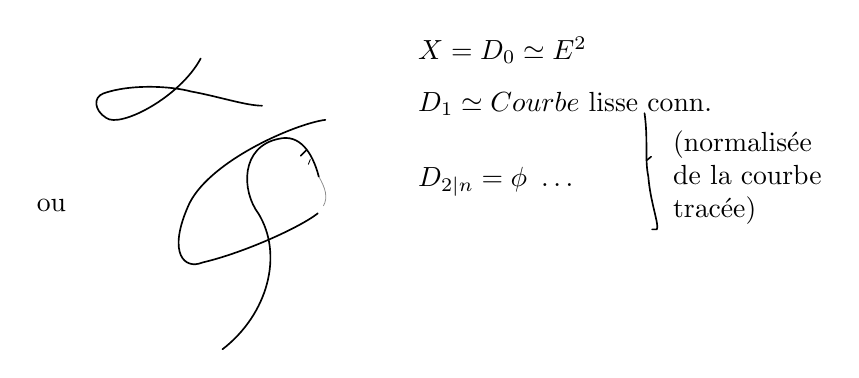
\begin{tikzpicture}[x=.012cm,y=-.012cm,line cap=round,line join=round]
\draw[line width=.6pt] (175,39)
  .. controls (153,80) and (90,113) .. (75,102)
  .. controls (62,94) and (61,80) .. (72,76)
  .. controls (100,66) and (143,68) .. (165,74)
  .. controls (193,79) and (223,89) .. (240,89);
\node at (17,195) {ou};
\draw[line width=.6pt] (307,104)
  .. controls (275,108) and (180,149) .. (161,197)
  .. controls (140,246) and (158,263) .. (177,255)
  .. controls (220,245) and (280,218) .. (299,203);
\draw[black!45,line width=.28pt] (305,195)
  .. controls (310,186) and (307,176) .. (300,164);
\draw[line width=.6pt] (300,164)
  .. controls (293,137) and (279,119) .. (258,124)
  .. controls (217,132) and (218,179) .. (236,203)
  .. controls (263,247) and (246,310) .. (198,347);
\draw[line width=.6pt] (287,136)--(281,142);
\draw[line width=.3pt] (291,146)--(289,151);
\node[anchor=base west] at (395,40) {$X=D_0\simeq\mathbb E^2$};
\node[anchor=base west] at (395,95) {$D_1\simeq\unsure{\text{Courbe}}$ \uline{lisse} conn.};
\node[anchor=base west] at (395,175) {$D_{\unsure{2|n}}=\phi\ \ldots$};
\draw[line width=.6pt] (645,97)
  .. controls (649,126) and (645,145) .. (649,164)
  .. controls (651,191) and (661,216) .. (658,220)--(653,220);
\draw[line width=.6pt] (647,147)--(652,143);
\node[anchor=north west,align=left] at (665,105) {(normalisée\\de la courbe\\tracée)};
\end{tikzpicture}}
qui ne peut être décrit par la donnée d'un diviseur sur $X$, \deleted{Lorsqu'on \unsure{en a choisi|a un \illegible{2}}}

\deleted{tel diviseur, dans}

L'opération de $\mathfrak S_d$ sur $\mathbb Z^d$ permet de construire sur $D_d$ un système local
\[
(183)\qquad T_d=D_d^!\mathbin\wedge_{(\mathfrak S_d)_{D_d}}(\mathbb Z^d)_{D_d},
\]
\deleted{\unsure{ou}} qui donne naissance à un groupe analytique (et $=$ algébrique) relatif sur $D_d$:
\[
(184)\qquad G_d=T_d\otimes_{\mathbb Z}{\mathbb G_m}_{D_d}\simeq D_d^d\mathbin\wedge_{(\mathfrak S_d)_{D_d}}\mathbb G_m^d
\]
\deleted{Enfin} et $T_d$ s'interprète en termes de $G_d$ comme le syst. local des $\unsure{\Pi_1|\pi_1}$ ou $H_1$ des fibres.
\margin{120}
